\subsection{Ejemplo teórico: espectro rotacional del HCl y del CO}

Para ilustrar la aplicación práctica de las deducciones teóricas, se analizará el caso de dos moléculas diatómicas ampliamente estudiadas en espectroscopía de microondas: el cloruro de hidrógeno (HCl) y el monóxido de carbono (CO). Ambas son moléculas lineales, pero difieren en su polaridad y, por tanto, en su comportamiento espectroscópico.

\subsubsection*{Constantes rotacionales y niveles de energía}

La constante rotacional \( B \) se determina a partir del momento de inercia \( I = \mu r^2 \), siendo \(\mu\) la masa reducida y \(r\) la distancia internuclear. Para el HCl y el CO se tienen los siguientes valores experimentales \cite{hollas2004modern,bernath2016spectra}:

\begin{table}[H]
\centering
\caption{Constantes rotacionales de HCl y CO.}
\begin{tabular}{lcc}
\hline
Molécula & \(B/hc\) (cm\(^{-1}\)) & \(r_e\) (Å) \\
\hline
HCl & 10.59341 & 1.27455 \\
CO  & 1.92253  & 1.12832 \\
\hline
\end{tabular}
\end{table}

A partir del modelo del rotor rígido, los niveles de energía están dados por:
\[
E_J = B J (J + 1),
\]
y las transiciones permitidas obedecen a la regla de selección \(\Delta J = \pm 1\), generando líneas espectrales igualmente espaciadas con separación:
\[
\Delta E = 2B(J + 1),
\qquad
\nu_{J \to J+1} = \frac{\Delta E}{h} = 2B(J + 1).
\]

\subsubsection*{Ejemplo numérico para HCl}

Para \(B = 10.59341~\text{cm}^{-1}\), la frecuencia de la primera transición (\(J=0 \to 1\)) es:
\[
\nu_{01} = 2B = 21.18682~\text{cm}^{-1} = 635.3~\text{GHz},
\]
correspondiente a una longitud de onda de aproximadamente \(0.472~\text{mm}\), dentro de la región de las microondas.

En general, las líneas aparecen en posiciones igualmente espaciadas de \(2B\), lo que produce un patrón característico en el espectro rotacional.

\begin{figure}[H]
\centering
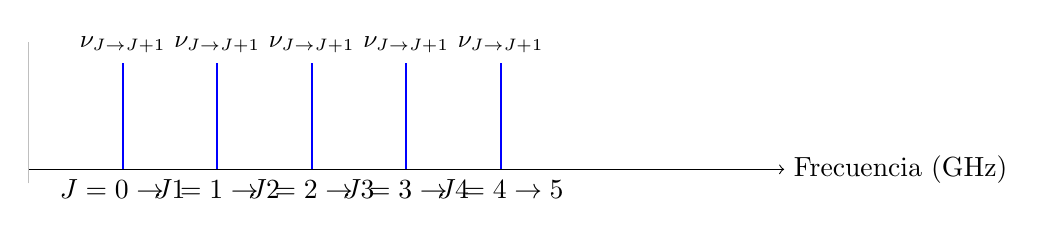
\begin{tikzpicture}[xscale=1.2,yscale=0.9]
  \draw[->] (0,0) -- (8,0) node[right]{Frecuencia (GHz)};
  \foreach \x/\label in {1/635,2/1270,3/1905,4/2540,5/3175}
    \draw[thick,blue] (\x,0) -- (\x,1.5)
    node[above,black]{\small $\nu_{J\to J+1}$};
  \draw[gray!50] (0,-0.2) -- (0,1.8);
  \node[below] at (1,0){$J=0\to1$};
  \node[below] at (2,0){$J=1\to2$};
  \node[below] at (3,0){$J=2\to3$};
  \node[below] at (4,0){$J=3\to4$};
  \node[below] at (5,0){$J=4\to5$};
\end{tikzpicture}
\caption{Espectro rotacional teórico del HCl. Las líneas están separadas por $2B$, correspondientes a las transiciones $J\to J+1$.}
\end{figure}

\subsubsection*{Comparación con CO y efecto de la polaridad}

En el caso del CO, aunque es una molécula diatómica heteronuclear, su momento dipolar es pequeño (\(\mu = 0.112~\text{D}\)), lo que reduce la intensidad de las transiciones rotacionales. Para moléculas homonucleares (como N\(_2\) o O\(_2\)), el momento dipolar permanente es nulo, y por lo tanto no se observan espectros de microondas.

El valor menor de \(B\) en CO implica un momento de inercia mayor y, por tanto, líneas más cercanas entre sí:
\[
\Delta \nu = 2B = 2 \times 1.92253~\text{cm}^{-1} = 115.1~\text{GHz}.
\]

\begin{figure}[H]
\centering
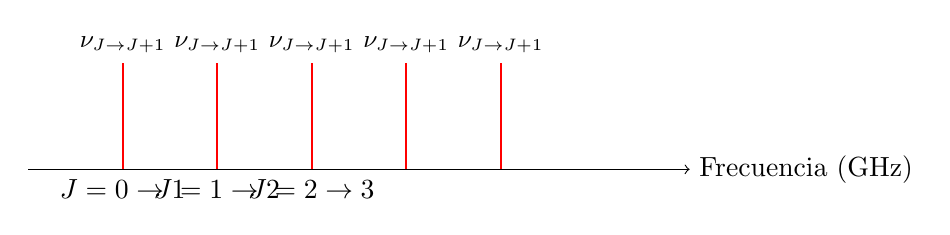
\begin{tikzpicture}[xscale=1.2,yscale=0.9]
  \draw[->] (0,0) -- (7,0) node[right]{Frecuencia (GHz)};
  \foreach \x/\label in {1/115,2/230,3/345,4/460,5/575}
    \draw[thick,red] (\x,0) -- (\x,1.5)
    node[above,black]{\small $\nu_{J\to J+1}$};
  \node[below] at (1,0){$J=0\to1$};
  \node[below] at (2,0){$J=1\to2$};
  \node[below] at (3,0){$J=2\to3$};
\end{tikzpicture}
\caption{Espectro rotacional teórico del CO, con líneas más cercanas debido a su menor constante rotacional.}
\end{figure}

\subsection*{Interpretación y aplicaciones}

El espaciado regular entre líneas rotacionales proporciona una vía directa para determinar \(B\) y, en consecuencia, el momento de inercia \(I\) y la distancia internuclear \(r\). Esta metodología constituye la base de la \textbf{determinación espectroscópica de estructuras moleculares}.

En astrofísica, las transiciones rotacionales del CO, HCN y HCO\(^+\) son observadas en el rango de 80–700~GHz, siendo empleadas para inferir la composición, temperatura y densidad de nubes moleculares interestelares \cite{bernath2016spectra}. El CO, en particular, es uno de los trazadores más usados para detectar regiones de formación estelar.

\begin{figure}[H]
\centering
\includegraphics[width=0.8\textwidth]{co_spectrum_radio.png}
\caption{Espectro rotacional observado del CO en el rango de microondas (ALMA Observatory, adaptado de \cite{bernath2016spectra}).}
\end{figure}

La espectroscopía de microondas, por tanto, trasciende el laboratorio y se convierte en una herramienta fundamental en la \textbf{física molecular, la astroquímica y la espectroscopía cuántica aplicada}, conectando la teoría rotacional con observaciones experimentales y astronómicas de alta precisión.

\subsection*{Interpretación y aplicaciones}

El espaciado regular entre líneas rotacionales proporciona una vía directa para determinar \(B\) y, en consecuencia, el momento de inercia \(I\) y la distancia internuclear \(r\). Esta metodología constituye la base de la \textbf{determinación espectroscópica de estructuras moleculares}.

En astrofísica, las transiciones rotacionales del CO, HCN y HCO\(^+\) son observadas en el rango de 80–700~GHz, siendo empleadas para inferir la composición, temperatura y densidad de nubes moleculares interestelares \cite{bernath2016spectra}. El CO, en particular, es uno de los trazadores más usados para detectar regiones de formación estelar.


La espectroscopía de microondas, por tanto, trasciende el laboratorio y se convierte en una herramienta fundamental en la \textbf{física molecular, la astroquímica y la espectroscopía cuántica aplicada}, conectando la teoría rotacional con observaciones experimentales y astronómicas de alta precisión.